\section{Test}\label{sec:test}
I test sono stati condotti su un dataset composto da 10.000 fino a 10.000.000 di email, considerando probabilità di
falsi positivi pari a 0,10, 0,05 e 0,01.
Per una valutazione preliminare dei tempi di esecuzione, dello speedup e del False Positive Rate (FPR),
focalizziamo l'attenzione sul valore di 0,05 per il FPR\@.

Gli altri valori di FPR sono riportati nell'appendice~\ref{sec:appendice}.

Il numero di processi considerati varia da 1 (modalità sequenziale) al massimo numero di processi disponibili sulla
macchina, ossia 16.
Le email sono state generate casualmente attraverso il generatore di email presente nel file \texttt{email\_generator.py}.
Poiché i test coprono un intervallo da 10.000 a 10.000.000 di email, il numero di funzioni hash è approssimativamente
pari a 5, e le dimensioni del vettore di bit variano da un minimo di 62.353 a un massimo di 62.352.243.

\subsection{OpenMP}\label{subsec:openmp-test}
\subsubsection{Setup}\label{subsubsec:openmp-setup}
\begin{figure}[H]
    \centering
    \minipage{0.49\textwidth}
    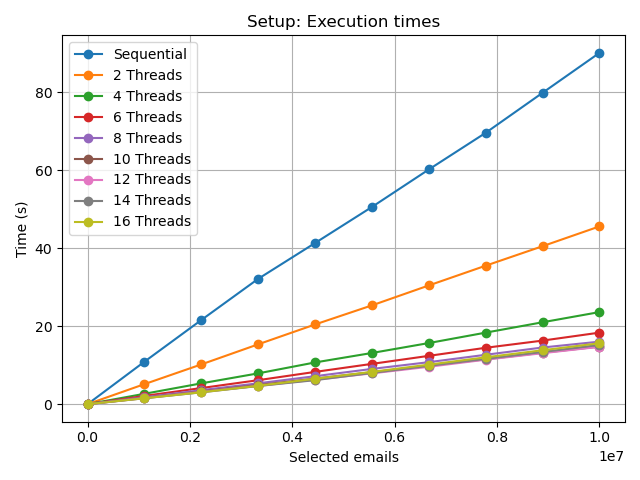
\includegraphics[width=\linewidth]{openmp/005/setup_times}
        \caption{Time setup Omp}\label{fig:005-setup_time_omp}
    \endminipage\hfill
    \minipage{0.49\textwidth}
    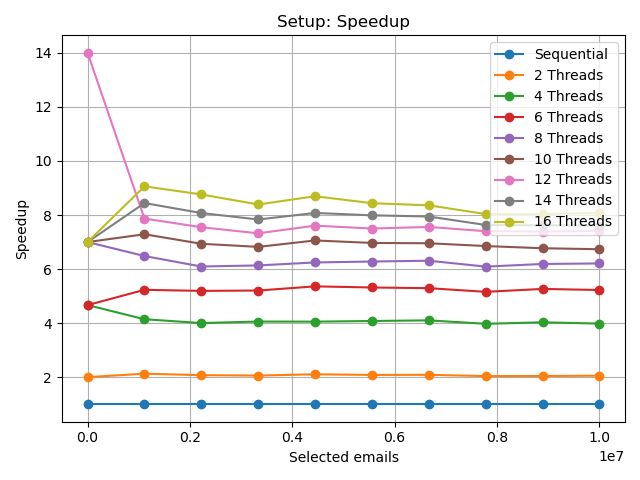
\includegraphics[width=\linewidth]{openmp/005/setup_speedup}
        \caption{Speedup setup Omp}\label{fig:005-setup_speedup_omp}
    \endminipage\hfill
\end{figure}
\begin{figure}[H]
    \centering
    \minipage{0.49\textwidth}
    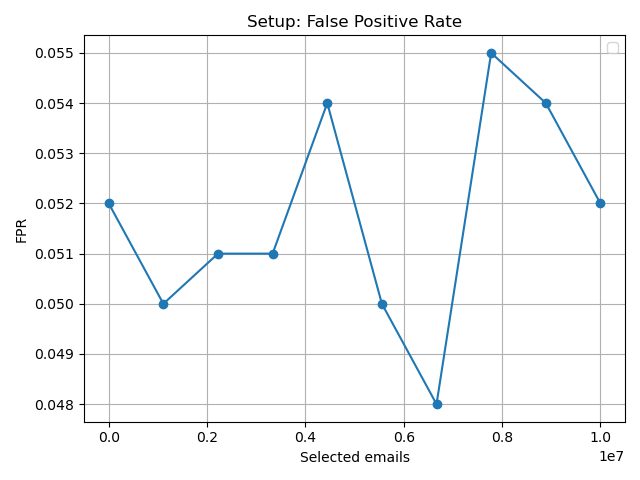
\includegraphics[width=\linewidth]{openmp/005/setup_fpr}
        \caption{FPR setup Omp}\label{fig:005-setup_fpr_omp}
    \endminipage\hfill
\end{figure}

Nell'analisi del tempo di esecuzione e dello speedup, emerge chiaramente come incrementando il numero di processi,
il tempo di esecuzione diminuisce significativamente rispetto alla versione sequenziale, raggiungendo un massimo di 9
con l'utilizzo di 16 processi.
È osservabile che all'aumentare del numero di processi, l'incremento dello speedup presenta una riduzione,
stabilizzandosi al valore di 8.
Per quanto concerne il False Positive Rate, i risultati ottenuti si collocano attorno al valore di FPR del 0,05, cioè
il valore per il quale è stato configurato per il BloomFilter.

\subsubsection{Filter}\label{subsubsec:fpr-005-filter}
\begin{figure}[H]
    \centering
    \minipage{0.49\textwidth}
    \includegraphics[width=\linewidth]{openmp/005/filter1_times}
        \caption{Time Filter Omp}\label{fig:005-filter_time_omp}
    \endminipage\hfill
    \minipage{0.49\textwidth}
    \includegraphics[width=\linewidth]{openmp/005/filter1_speedup}
        \caption{Speedup Filter Omp}\label{fig:005-filter_speedup_omp}
    \endminipage\hfill
\end{figure}
\begin{figure}[H]
    \centering
    \minipage{0.49\textwidth}
    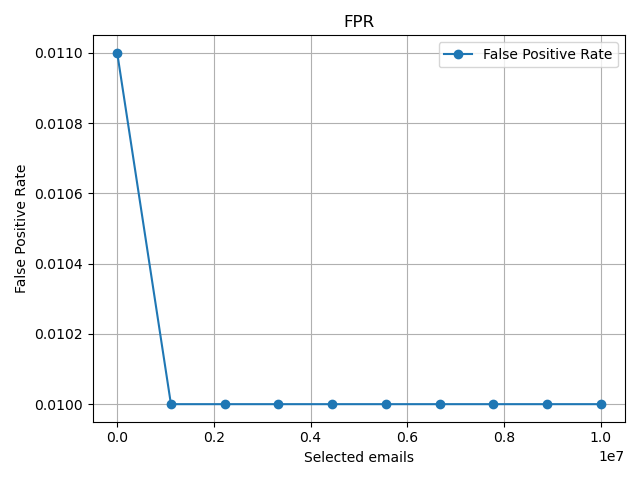
\includegraphics[width=\linewidth]{openmp/005/filter_fpr}
        \caption{FPR Filter Omp}\label{fig:005-filter_fpr_omp}
    \endminipage\hfill
\end{figure}

Analogamente alla fase di setup, nell'incrementare il numero di processi, si osserva una significativa riduzione del
tempo di esecuzione rispetto alla modalità sequenziale, con un picco massimo di 11 utilizzando 16 processi.
In questa circostanza, tuttavia, la diminuzione dello speedup, al variare dei processi, non è altrettanto marcata
rispetto alla fase di setup.
Il valore di FPR raggiunge una sorta di plateau una volta che un numero sufficiente di email è stato raggiunto.

\subsubsection{Confronto Filter}\label{subsubsec:confronto-filter}
Qui vengono esaminate le differenze tra le due versioni implementate del filtro.

\begin{figure}[H]
    \centering
    \minipage{0.49\textwidth}
    \includegraphics[width=\linewidth]{openmp/filters-005/filter1_times}
        \caption{Time Filter 1}\label{fig:005-filter1_time_omp}
    \endminipage\hfill
    \minipage{0.49\textwidth}
    \includegraphics[width=\linewidth]{openmp/filters-005/filter1_speedup}
        \caption{Speedup Filter 1}\label{fig:005-filter1_speedup_omp}
    \endminipage\hfill
\end{figure}
\begin{figure}[H]
    \centering
    \minipage{0.49\textwidth}
    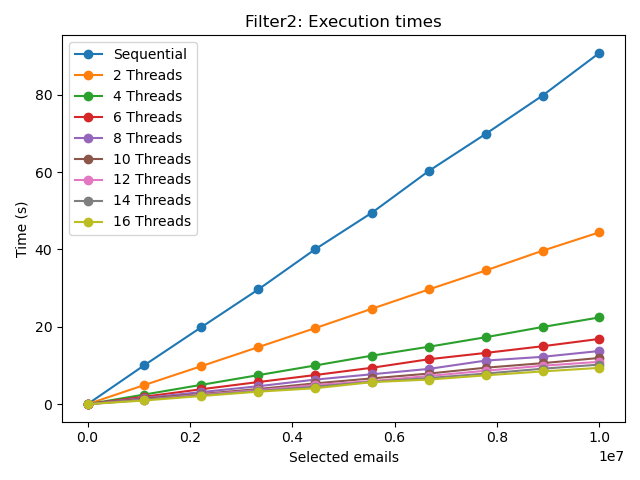
\includegraphics[width=\linewidth]{openmp/filters-005/filter2_times}
        \caption{Time Filter 2}\label{fig:005-filter2_time_omp}
    \endminipage\hfill
    \minipage{0.49\textwidth}
    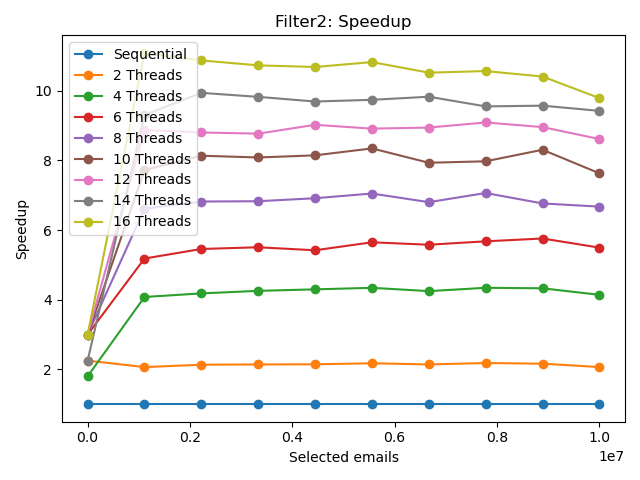
\includegraphics[width=\linewidth]{openmp/filters-005/filter2_speedup}
        \caption{Speedup Filter 2}\label{fig:005-filter2_speedup_omp}
    \endminipage\hfill
\end{figure}

Come evidente, le due versioni del filtro mostrano performance praticamente identiche sia in termini di tempo di
esecuzione che di speedup.
Pertanto, a causa di questa similitudine prestazionale, prenderemo in considerazione la prima implementazione per
le analisi successive.

\subsection{Joblib}\label{subsec:joblib-test}
\subsubsection{Setup}\label{subsubsec:joblib-setup}
\begin{figure}[H]
    \centering
    \minipage{0.49\textwidth}
    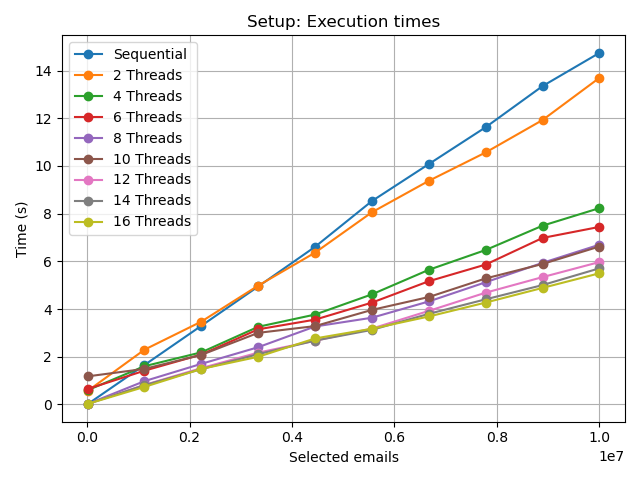
\includegraphics[width=\linewidth]{joblib/005/setup_time_plot}
        \caption{Time setup Joblib}\label{fig:005-setup_time_joblib}
    \endminipage\hfill
    \minipage{0.49\textwidth}
    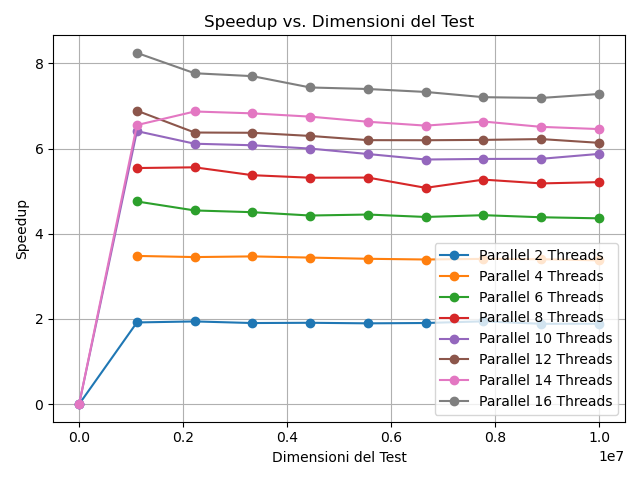
\includegraphics[width=\linewidth]{joblib/005/setup_speedup_plot}
        \caption{Speedup setup Joblib}\label{fig:005-setup_speedup_joblib}
    \endminipage\hfill
\end{figure}
\begin{figure}[H]
    \centering
    \minipage{0.49\textwidth}
    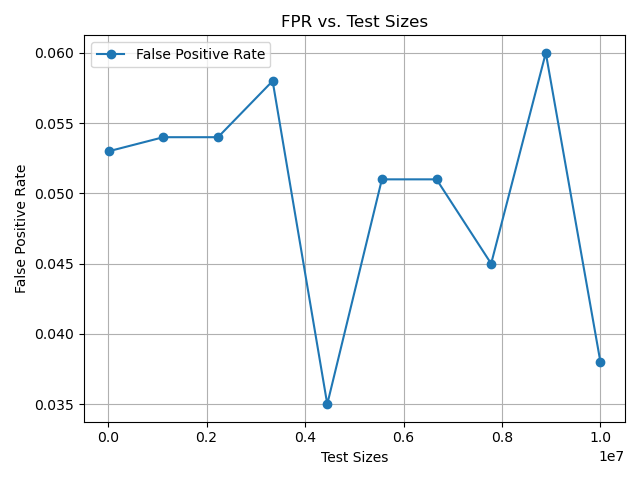
\includegraphics[width=\linewidth]{joblib/005/setup_fpr_plot}
        \caption{FPR setup Joblib}\label{fig:005-setup_fpr_joblib}
    \endminipage\hfill
\end{figure}

I risultati ottenuti nella fase di setup con la versione Joblib evidenziano come l'aumento del numero di processori
conduca a una riduzione del tempo di esecuzione, seppur in maniera meno significativa rispetto alla versione OpenMP\@.
Lo speedup risulta notevole e superiormente performante rispetto alla versione sequenziale una volta che un certo numero
di email è stato raggiunto.
Questo fenomeno è attribuibile al tempo di virtualizzazione dei processi, che in questo caso incide negativamente sul
tempo di esecuzione per un numero ridotto di email.
Il valore massimo di speedup raggiunto si assesta intorno a 2.7.
Anche in questo caso, i valori di FPR (False Positive Rate) si collocano attorno al valore di 0.05.

\subsubsection{Filter}\label{subsubsec:joblib-filter}
\begin{figure}[H]
    \centering
    \minipage{0.49\textwidth}
    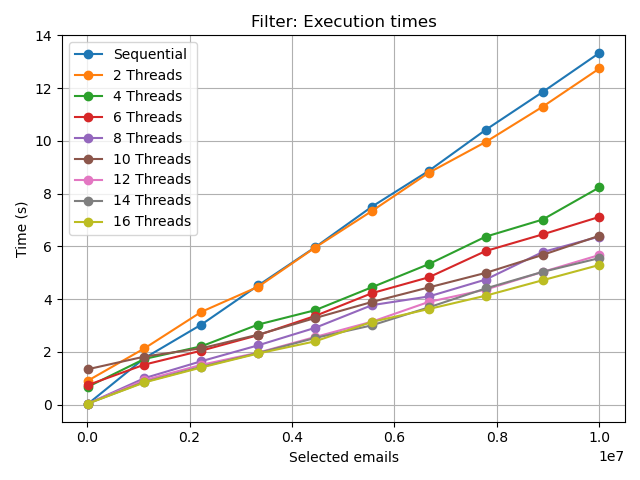
\includegraphics[width=\linewidth]{joblib/005/filter_time_plot}
        \caption{Time Filter Joblib}\label{fig:005-filter_time_joblib}
    \endminipage\hfill
    \minipage{0.49\textwidth}
    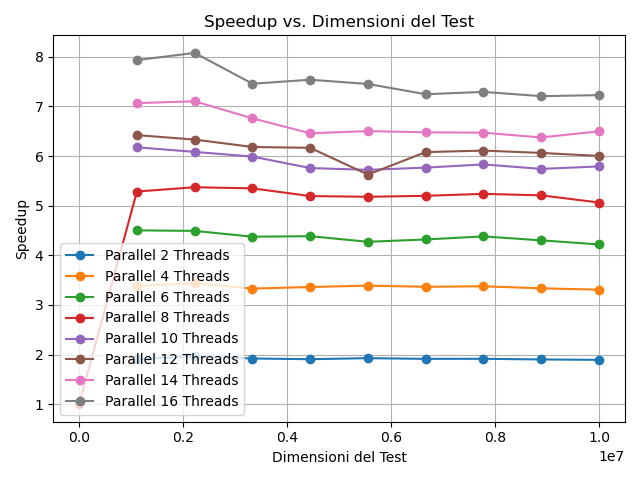
\includegraphics[width=\linewidth]{joblib/005/filter_speedup_plot}
        \caption{Speedup Filter Joblib}\label{fig:005-filter_speedup_joblib}
    \endminipage\hfill
\end{figure}
\begin{figure}[H]
    \centering
    \minipage{0.49\textwidth}
    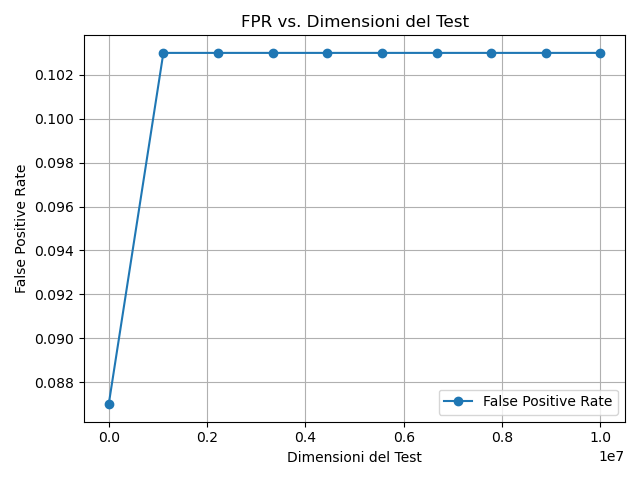
\includegraphics[width=\linewidth]{joblib/005/filter_fpr_plot}
        \caption{FPR Filter Joblib}\label{fig:005-filter_fpr_joblib}
    \endminipage\hfill
\end{figure}

Anche nella fase di filtraggio, come nella fase di setup, l'aumento del numero di processi conduce a una riduzione del
tempo di esecuzione, seppur in maniera meno significativa rispetto alla versione OpenMP\@.
Infatti il valore massimo di speedup raggiunto si assesta intorno a 2.5.
Una volta che un certo numero di email è stato raggiunto, il valore di FPR si stabilizza attorno al valore di 0.05.

\subsubsection{Chunks}\label{subsubsec:005-chunks}
Ora esamineremo la possibilità di eseguire un'operazione di chunking più estesa rispetto al numero di thread disponibili
nella fase di setup per valutare se è possibile migliorare le prestazioni.
I valori di riferimento per i chunk sono 16, 32, 64, 128, 256, 512, 1024, 2048.

\begin{figure}[H]
    \centering
    \minipage{0.49\textwidth}
    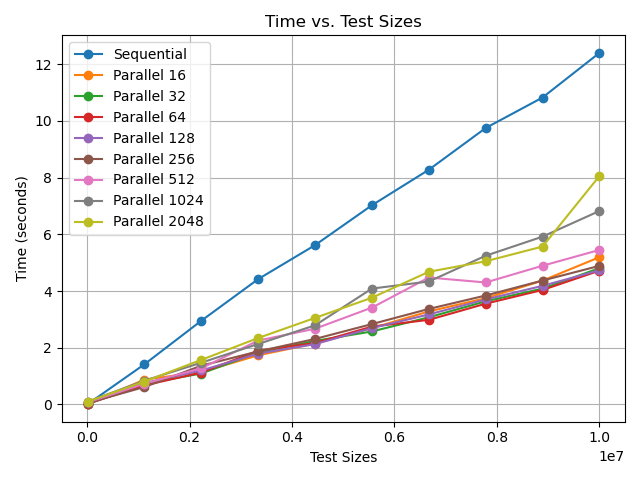
\includegraphics[width=\linewidth]{joblib/005/chunks_time_plot}
        \caption{Times setup Chunks}\label{fig:005-chunks_time}
    \endminipage\hfill
    \minipage{0.49\textwidth}
    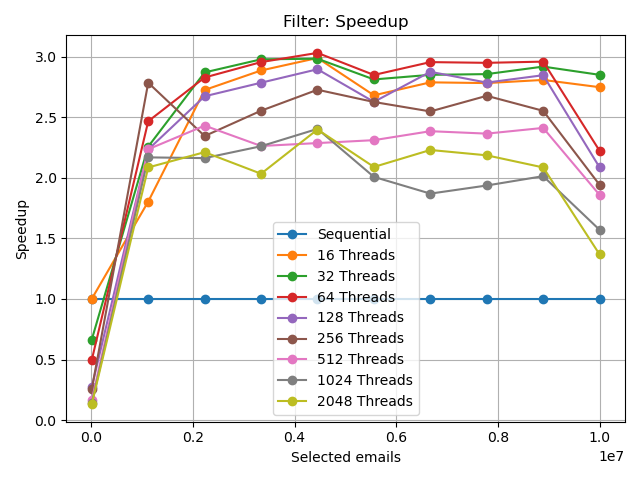
\includegraphics[width=\linewidth]{joblib/005/chunks_speedup_plot}
        \caption{Speedup setup Chunks}\label{fig:005-chunks_speedup}
    \endminipage\hfill
\end{figure}

I risultati ottenuti suggeriscono che l'implementazione dell'operazione di chunking ha portato a miglioramenti
sostanziali nelle performance di speedup.
In particolare, l'aumento del numero di chunk ha contribuito a un notevole miglioramento dello speedup,
raggiungendo un massimo di 3.
Tuttavia, oltre una soglia di 64 chunk, si è verificato un declino nelle performance.

\subsection{Confronto}\label{subsec:confronto}
\subsection{Setup}\label{subsec:confronto-setup}
Nel test di configurazione iniziale, è evidente che la versione sviluppata con OpenMP presenta una performance temporale
inferiore rispetto alla sua controparte.
Al contrario, in termini di speedup, la versione OpenMP supera quella sviluppata con Joblib,
raggiungendo uno speedup massimo di 2.70 nella versione Joblib e 9 nella versione OpenMP,
sfruttando il massimo numero di thread disponibili.

\subsection{Filter}\label{subsec:confronto-filter}
Nel test di filtraggio, è evidente che la versione sviluppata con OpenMP presenta una performance temporale inferiore
rispetto alla sua controparte.
Tuttavia, in termini di speedup, la versione OpenMP supera quella sviluppata con Joblib, raggiungendo un massimo di 11
nella versione OpenMP e 2.5 nella versione Joblib, sfruttando il massimo numero di thread disponibili.
I valori di FPR (False Positive Rate) sono praticamente identici tra le due versioni.



